\documentclass[12pt]{article}
\usepackage[margin=1in]{geometry}
\usepackage[all]{xy}

\usepackage{amsmath,amsthm,amssymb,color,latexsym}
\usepackage{geometry}        
\geometry{letterpaper}    
\usepackage{graphicx}
\usepackage[utf8]{vietnam}
\newtheorem{problem}{Problem}
\usepackage{listings}
\usepackage{tcolorbox}
\usepackage{verbatim}
\usepackage{tabularx}
\usepackage{array}
\usepackage{colortbl}
\usepackage{xcolor}
\usepackage{float}
\usepackage{longtable}
\usepackage{hyperref}
\tcbuselibrary{skins}
\definecolor{Salmon}{RGB}{235,235,235}

\newcolumntype{Y}{>{\raggedleft\arraybackslash}X}

\definecolor{codegreen}{rgb}{0,0.6,0}
\definecolor{codegray}{rgb}{0.5,0.5,0.5}
\definecolor{codepurple}{rgb}{0.58,0,0.82}
\definecolor{backcolour}{rgb}{0.95,0.95,0.92}


\definecolor{blockbackgroundcolor}{RGB}{235,235,235}
\definecolor{blockbordercolor}{RGB}{79,79,79}
\newenvironment{solution}[1][\it{Answer}]{\textbf{#1. } }{}
\lstdefinestyle{mystyle}{
    backgroundcolor=\color{backcolour},   
    commentstyle=\color{codegreen},
    keywordstyle=\color{magenta},
    numberstyle=\tiny\color{codegray},
    stringstyle=\color{codepurple},
    basicstyle=\ttfamily\footnotesize,
    breakatwhitespace=false,         
    breaklines=true,                 
    captionpos=b,                    
    keepspaces=true,                 
    numbers=left,                    
    numbersep=5pt,                  
    showspaces=false,                
    showstringspaces=false,
    showtabs=false,                  
    tabsize=2
}

\tcbset{tab1/.style={fonttitle=\bfseries\large,fontupper=\normalsize\sffamily,
colback=yellow!10!white,colframe=red!75!black,colbacktitle=Salmon!40!white,
coltitle=black,center title,freelance,frame code={
\foreach \n in {north east,north west,south east,south west}
{\path [fill=red!75!black] (interior.\n) circle (3mm); };},}}

\tcbset{tab2/.style={enhanced,fonttitle=\bfseries,fontupper=\normalsize\sffamily,
colback=yellow!10!white,colframe=red!50!black,colbacktitle=Salmon!40!white,
coltitle=black,center title}}

\begin{document}
\graphicspath{ {Figs/} } 

\noindent Trí tuệ nhân tạo - CS106.O21 \hfill Solving Knapsack \\
Nguyễn Hoàng Tân - 21521413 \hfill  Google OR Tools 

\hrulefill


\begin{problem}
	Phân loại, phân tích các nhóm Test Instances
\end{problem}
Để có cái nhìn tổng quan về hiệu suất thuật toán knapsack, chúng ta sẽ thực hiện thí nghiệm trên 13 bộ test instance được giới thiệu tại section 5.5 trong quyển \href{https://github.com/Dev-Aligator/UIT/blob/master/CS106.O21/KnapsackORTools/vdoc.pub_knapsack-problems.pdf}{Hans Kellerer - Ulrich Pferschy David Pisinger Knapsack Problems}. 

Trong tất cả các trường hợp, trọng lượng mỗi món đồ được phân phối đều trong một khoảng R = 1000 và 10000. Giá trị được biểu diễn dưới dạng một hàm phụ thuộc vào trọng lượng, tạo ra các đặc tính cụ thể của mỗi nhóm. Các nhóm trường hợp được minh họa trong Hình \ref{fig:test_instances}. \\

\begin{figure}[H]
	\centering
	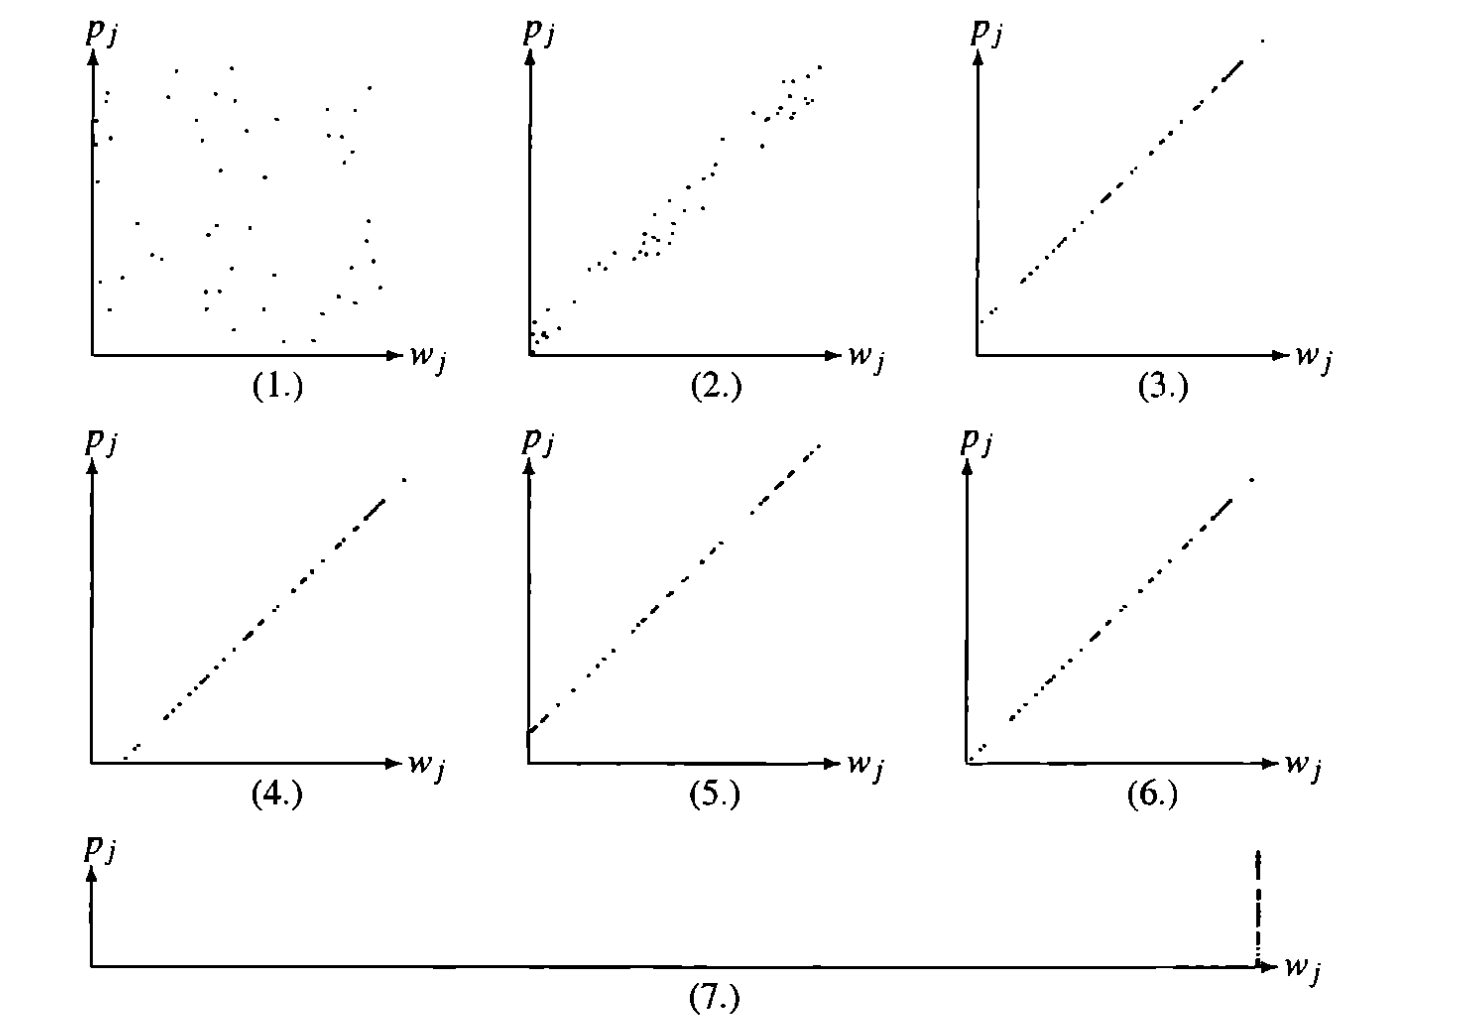
\includegraphics[scale=0.34]{Test_Instances_Fig.png}
	\caption{Classical test instances. (1.) Uncorrelated instances. (2.) Weakly correlated in-
	stances. (3.) Strongly correlated instances. (4.) Inverse strongly correlated instances. (5.) Al-
	most strongly correlated instances. (6.) Subset sum instances. (7.) Uncorrelated instances with
	similar weights. Note that instances (3.) and (5.) look very similar since the extra “noise" in
	almost strongly correlated instances is very small.}
	\label{fig:test_instances}
\end{figure}


\hspace{-1em}\textbf{1. Uncorrelated data instances (00Uncorrelated)} 

$W_j$ và $p_j$ được chọn ngẫu nhiên trong [1, R]. Trong những trường hợp này, không có sự tương quan giữa giá trị và trọng lượng của một mặt hàng. Các trường hợp này minh họa những tình huống mà việc giả định rằng giá trị không phụ thuộc vào trọng lượng là hợp lý. Các trường hợp không tương quan này thường dễ giải quyết, vì có sự biến thiên lớn giữa giá trị và trọng lượng.

\hspace{-1em}\textbf{2. Weakly correlated instances (01WeaklyCorrelated)} 

Trọng lượng $w_j$ được chọn ngẫu nhiên trong [1, R] và giá trị $p_j$ trong [$w_j - R / 10, w_j + R / 10$] sao cho $p_j \geq 1$. Mặc dù có tên là Weakly correlated, các trường hợp này có một tương quan rất cao giữa giá trị và trọng lượng của một mặt hàng. Thông thường, giá trị chênh lệch so với trọng lượng chỉ là một vài phần trăm. 

\hspace{-1em}\textbf{3. Strongly correlated instances (02StronglyCorrelated)} 

Các trường hợp dữ liệu tương quan mạnh: trọng lượng $w_j$ được phân phối trong [1, R] và $p_j = W_j +R/10$. Những trường hợp như vậy tương ứng với tình huống trong thực tế.

\hspace{-1em}\textbf{4. Inverse strongly correlated (03InverseStronglyCorrelated)} 
$p_j$ được phân phối trong khoảng [1,R] và $w_j = p_j + R/10.$ Đây là trường hợp tương tự nhưng ngược lại so với Strongly correlated.

\hspace{-1em}\textbf{4. Almost strongly correlated (04AlmostStronglyCorrelated)}

$w_j$ được phân phối trong khoảng [1,R] và $p_j$ nằm trong khoảng [$w_j + R/10 - R/500, w_j + R/10 + R/500$].

\hspace{-1em}\textbf{5. Subset sum (05SubsetSum)}

$w_j$ được phân phối ngẫu nhiên trong đoạn [1,R] và $p_j = w_j$. Đây là tình huống mà giá trị bằng (hoặc tỉ lệ thuận) với cân nặng của món hàng.

\hspace{-1em}\textbf{6. Uncorrelated with similar weights (06UncorrelatedWithSimilarWeights)}

$w_j$ nằm trong khoảng [100000,100100] và $p_j$ thì nằm trong khoảng [1,1000].

\hspace{-1em}\textbf{7. Spanner instance}

Tất cả món hàng là bội của một nhóm nhỏ các món hàng – vì thế nên mới có tên spanner (không gian sinh). Ta có hàm \textit{span(v,m)} được định nghĩa bởi 3 tham số:
\begin{enumerate}
    \item $v$: kích thước của tập spanner.
    \item $m$: giới hạn của bội số.
    \item Loại phân phối (uncorrelated, weakly correlated, strongly correlated, etc.).
\end{enumerate}

Một tập hợp gồm $v$ món hàng được khởi tạo với cân nặng nằm trong khoảng [1,R] và giá trị thì tuân theo phân phối. Món hàng $(p_k, w_k)$ trong không gian sinh được chọn và chuẩn hóa bằng cách chia $p$ và $w$ với $m + 1$. Bội số $a$ được chọn ngẫu nhiên trong khoảng [1,m], vì thế ta sẽ có món hàng mới với giá trị và cân nặng lần lượt là $(a \times p_k, a \times w_k)$.

Trong 3 tập \textit{07SpannerUncorrelated}, \textit{08SpannerWeaklyCorrelated} và \textit{09Spanner}, ta chọn $v = 2$ và $m = 10$.

\hspace{-1em}\textbf{8. Multiple strongly correlated (10MultipleStronglyCorrelated)}

Gồm 3 tham số là $k1$, $k2$ và $d$. Cân nặng của các món hàng được phân phối ngẫu nhiên trong khoảng [1,R]. Nếu $w_j$ chia hết cho $d$ thì $p_j = w_j + k1$, ngược lại thì $p_j = w_j + k2$. Trong instance này, $k1 = 3 \times R/10$, $k2 = 2 \times R/10$ và $d = 6$.

\hspace{-1em}\textbf{9. Profit Ceiling (11ProfitCeiling)}

Mọi giá trị $p$ đều là bội số của một tham số $d$ cho trước. Cân nặng $w$ được phân phối ngẫu nhiên trong khoảng [1,R] và $p_j = d\left[\frac{w_j}{d}\right]$. Trong đây ta chọn $d = 3$.

\hspace{-1em}\textbf{10. Circle (12Circle)}

Giá trị $p$ được sinh theo một hàm phụ thuộc vào cân nặng $w$ dưới dạng phương trình đường tròn (ellipsis). Cân nặng được phân phối đều theo khoảng [1,R] và với mỗi $w$ ta sẽ có một giá trị tương ứng $p = d\sqrt{4R^2 - (w - 2R)^2}$.


\begin{problem}
	Lập bảng kết quả
\end{problem}
\lstset{style=mystyle}
	Tiến hành load từng test instances và chạy thực nghiệm. Lưu ý, mỗi test case chỉ chạy tối đa 30s (set\_time\_limit) và ở mỗi range thuộc một nhóm và size nhất định sẽ chỉ chạy 2 test case đầu tiên\\


	\begin{tcolorbox}[boxrule=0.5pt, colback=white]
		\begin{lstlisting}[language=python, numbers=none, basicstyle=\ttfamily\footnotesize]
solver = knapsack_solver.KnapsackSolver(
         knapsack_solver.SolverType.KNAPSACK_MULTIDIMENSION_BRANCH_AND_BOUND_SOLVER,
         "KnapsackExample",
		)

time_limit = 30
solver.set_time_limit(time_limit)
		\end{lstlisting}
		\end{tcolorbox}


\begin{tcolorbox}[tab2,tabularx={X|Y|Y|Y|Y|Y|Y|Y},title=Bảng thống kê với từng Test Instances,boxrule=0.5pt]
	\textbf{Type} & \textbf{Size} & \textbf{Range} & \textbf{Name} & \textbf{Total Value} & \textbf{Total Weight} & \textbf{Running Time} & \textbf{Optimal Solution} \\
	\hline
04 & nn00200 & RR01000 &  s089 &  63650 &  49527 & 0.034 & True \\
04 & nn00200 & RR01000 &  s017 &  64928 &  51029 & 0.778 & True \\
04 & nn00200 & RR10000 &  s089 &  635994 &  494811 & 0.146 & True \\
04 & nn00200 & RR10000 &  s017 &  648850 &  509848 & 3.638 & True \\
04 & nn10000 & RR01000 &  s089 &  3180114 &  2475166 & 29.711 & True \\
04 & nn10000 & RR01000 &  s017 &  3173001 &  2469901 & 29.402 & True \\
04 & nn10000 & RR10000 &  s089 &  31774942 &  24725069 & 29.503 & True \\
04 & nn10000 & RR10000 &  s017 &  31710728 &  24678021 & 0.015 & True \\
04 & nn00500 & RR01000 &  s089 &  160529 &  125430 & 29.999 & True \\
04 & nn00500 & RR01000 &  s017 &  156217 &  120681 & 29.448 & True \\
04 & nn00500 & RR10000 &  s089 &  1604253 &  1253201 & 29.53 & True \\
04 & nn00500 & RR10000 &  s017 &  1560960 &  1205714 & 29.398 & True \\
04 & nn05000 & RR01000 &  s089 &  1589318 &  1237047 & 6.835 & True \\
04 & nn05000 & RR01000 &  s017 &  1593223 &  1243024 & 29.667 & True \\
04 & nn05000 & RR10000 &  s089 &  15877191 &  12354649 & 29.754 & True \\
04 & nn05000 & RR10000 &  s017 &  15922383 &  12419788 & 29.721 & True \\
04 & nn00100 & RR01000 &  s089 &  32101 &  24988 & 0.618 & True \\
04 & nn00100 & RR01000 &  s017 &  33521 &  26615 & 1.488 & True \\
04 & nn00100 & RR10000 &  s089 &  320721 &  249644 & 2.071 & True \\
04 & nn00100 & RR10000 &  s017 &  334994 &  265939 & 7.185 & True \\
04 & nn02000 & RR01000 &  s089 &  634219 &  492957 & 29.894 & True \\
04 & nn02000 & RR01000 &  s017 &  637974 &  497240 & 29.776 & True \\
04 & nn02000 & RR10000 &  s089 &  6337730 &  4925064 & 29.508 & True \\
04 & nn02000 & RR10000 &  s017 &  6372482 &  4965280 & 29.436 & True \\
04 & nn00050 & RR01000 &  s089 &  16709 &  13208 & 0.0 & True \\
04 & nn00050 & RR01000 &  s017 &  17479 &  14070 & 0.001 & True \\
04 & nn00050 & RR10000 &  s089 &  166973 &  131954 & 0.0 & True \\
04 & nn00050 & RR10000 &  s017 &  174676 &  140598 & 0.002 & True \\
04 & nn01000 & RR01000 &  s089 &  318449 &  247948 & 29.997 & True \\
04 & nn01000 & RR01000 &  s017 &  315521 &  244792 & 29.357 & True \\
04 & nn01000 & RR10000 &  s089 &  3181797 &  2476813 & 29.375 & True \\
04 & nn01000 & RR10000 &  s017 &  3154093 &  2446984 & 29.483 & True \\
12 & nn00200 & RR01000 &  s089 &  1043581 &  49527 & 0.126 & True \\
12 & nn00200 & RR01000 &  s017 &  1075229 &  51029 & 0.061 & True \\
12 & nn00200 & RR10000 &  s089 &  32985928 &  494814 & 1.162 & True \\
12 & nn00200 & RR10000 &  s017 &  33988279 &  509850 & 29.905 & True \\
12 & nn10000 & RR01000 &  s089 &  52154349 &  2475179 & 27.984 & True \\
12 & nn10000 & RR01000 &  s017 &  52046402 &  2470057 & 29.476 & True \\
12 & nn10000 & RR10000 &  s089 &  1648577961 &  24729920 & 29.673 & True \\
12 & nn10000 & RR10000 &  s017 &  1645118204 &  24678021 & 29.586 & True \\
12 & nn00500 & RR01000 &  s089 &  2642927 &  125430 & 29.861 & True \\
12 & nn00500 & RR01000 &  s017 &  2542862 &  120681 & 28.374 & True \\
12 & nn00500 & RR10000 &  s089 &  83542774 &  1253205 & 28.622 & True \\
12 & nn00500 & RR10000 &  s017 &  80376862 &  1205714 & 28.645 & True \\
12 & nn05000 & RR01000 &  s089 &  26065737 &  1237047 & 28.507 & True \\
\end{tcolorbox}


\begin{tcolorbox}[tab2,tabularx={X|Y|Y|Y|Y|Y|Y|Y},title=Bảng thống kê với từng Test Instances,boxrule=0.5pt]
	\textbf{Type} & \textbf{Size} & \textbf{Range} & \textbf{Name} & \textbf{Total Value} & \textbf{Total Weight} & \textbf{Running Time} & \textbf{Optimal Solution} \\
	\hline
12 & nn05000 & RR01000 &  s017 &  26198391 &  1243343 & 29.818 & True \\
12 & nn05000 & RR10000 &  s089 &  823931403 &  12359596 & 29.682 & True \\
12 & nn05000 & RR10000 &  s017 &  828104584 &  12422197 & 29.64 & True \\
12 & nn00100 & RR01000 &  s089 &  526521 &  24988 & 16.014 & True \\
12 & nn00100 & RR01000 &  s017 &  560803 &  26615 & 29.39 & True \\
12 & nn00100 & RR10000 &  s089 &  16642622 &  249652 & 12.796 & True \\
12 & nn00100 & RR10000 &  s017 &  17728703 &  265944 & 1.229 & True \\
12 & nn02000 & RR01000 &  s089 &  10387061 &  492957 & 0.002 & True \\
12 & nn02000 & RR01000 &  s017 &  10481189 &  497424 & 29.995 & True \\
12 & nn02000 & RR10000 &  s089 &  328332524 &  4925237 & 29.462 & True \\
12 & nn02000 & RR10000 &  s017 &  331301437 &  4969773 & 29.668 & True \\
12 & nn00050 & RR01000 &  s089 &  278305 &  13208 & 0.765 & True \\
12 & nn00050 & RR01000 &  s017 &  296489 &  14071 & 0.99 & True \\
12 & nn00050 & RR10000 &  s089 &  8797486 &  131969 & 0.219 & True \\
12 & nn00050 & RR10000 &  s017 &  9372992 &  140602 & 0.154 & True \\
12 & nn01000 & RR01000 &  s089 &  5224498 &  247948 & 29.986 & True \\
12 & nn01000 & RR01000 &  s017 &  5165287 &  245138 & 28.207 & True \\
12 & nn01000 & RR10000 &  s089 &  165147517 &  2477338 & 29.278 & True \\
12 & nn01000 & RR10000 &  s017 &  163269936 &  2449173 & 29.362 & True \\
00 & nn00200 & RR01000 &  s089 &  80555 &  51097 & 0.0 & True \\
00 & nn00200 & RR01000 &  s017 &  83156 &  47781 & 0.0 & True \\
00 & nn00200 & RR10000 &  s089 &  804990 &  510421 & 0.0 & True \\
00 & nn00200 & RR10000 &  s017 &  830970 &  477181 & 0.0 & True \\
00 & nn10000 & RR01000 &  s089 &  4049025 &  2474102 & 0.0 & True \\
00 & nn10000 & RR01000 &  s017 &  4032422 &  2469230 & 0.013 & True \\
00 & nn10000 & RR10000 &  s089 &  40467150 &  24718848 & 0.005 & True \\
00 & nn10000 & RR10000 &  s017 &  40300050 &  24670348 & 0.001 & True \\
00 & nn00500 & RR01000 &  s089 &  205159 &  122517 & 0.0 & True \\
00 & nn00500 & RR01000 &  s017 &  197873 &  124445 & 0.0 & True \\
00 & nn00500 & RR10000 &  s089 &  2050450 &  1224048 & 0.0 & True \\
00 & nn00500 & RR10000 &  s017 &  1977628 &  1243406 & 0.0 & True \\
00 & nn05000 & RR01000 &  s089 &  2022297 &  1238131 & 0.001 & True \\
00 & nn05000 & RR01000 &  s017 &  2020478 &  1226713 & 0.004 & True \\
00 & nn05000 & RR10000 &  s089 &  20211524 &  12370320 & 0.0 & True \\
00 & nn05000 & RR10000 &  s017 &  20192624 &  12255824 & 0.002 & True \\
00 & nn00100 & RR01000 &  s089 &  41562 &  24536 & 0.0 & True \\
00 & nn00100 & RR01000 &  s017 &  43703 &  24374 & 0.0 & True \\
00 & nn00100 & RR10000 &  s089 &  415339 &  245080 & 0.0 & True \\
00 & nn00100 & RR10000 &  s017 &  436863 &  243850 & 0.0 & True \\
00 & nn02000 & RR01000 &  s089 &  808000 &  497774 & 0.0 & True \\
00 & nn02000 & RR01000 &  s017 &  807210 &  495607 & 0.0 & True \\
00 & nn02000 & RR10000 &  s089 &  8075481 &  4973419 & 0.004 & True \\
\end{tcolorbox}

\begin{tcolorbox}[tab2,tabularx={X|Y|Y|Y|Y|Y|Y|Y},title=Bảng thống kê với từng Test Instances,boxrule=0.5pt]
	\textbf{Type} & \textbf{Size} & \textbf{Range} & \textbf{Name} & \textbf{Total Value} & \textbf{Total Weight} & \textbf{Running Time} & \textbf{Optimal Solution} \\
	\hline
00 & nn02000 & RR10000 &  s017 &  8067384 &  4951511 & 0.001 & True \\
00 & nn00050 & RR01000 &  s089 &  22773 &  11660 & 0.0 & True \\
00 & nn00050 & RR01000 &  s017 &  22989 &  12530 & 0.0 & True \\
00 & nn00050 & RR10000 &  s089 &  227570 &  116461 & 0.0 & True \\
00 & nn00050 & RR10000 &  s017 &  229750 &  125176 & 0.0 & True \\
00 & nn01000 & RR01000 &  s089 &  409464 &  245002 & 0.001 & True \\
00 & nn01000 & RR01000 &  s017 &  398503 &  252286 & 0.0 & True \\
00 & nn01000 & RR10000 &  s089 &  4092529 &  2447884 & 0.0 & True \\
00 & nn01000 & RR10000 &  s017 &  3982790 &  2520561 & 0.0 & True \\
11 & nn00200 & RR01000 &  s089 &  49506 &  49527 & 0.119 & True \\
11 & nn00200 & RR01000 &  s017 &  51009 &  51028 & 28.116 & True \\
11 & nn00200 & RR10000 &  s089 &  494796 &  494814 & 12.472 & True \\
11 & nn00200 & RR10000 &  s017 &  509829 &  509849 & 29.314 & True \\
11 & nn10000 & RR01000 &  s089 &  2474226 &  2475179 & 28.509 & True \\
11 & nn10000 & RR01000 &  s017 &  2469147 &  2470057 & 29.734 & True \\
11 & nn10000 & RR10000 &  s089 &  24728979 &  24729918 & 29.766 & True \\
11 & nn10000 & RR10000 &  s017 &  24677049 &  24678021 & 29.777 & True \\
11 & nn00500 & RR01000 &  s089 &  125382 &  125428 & 29.911 & True \\
11 & nn00500 & RR01000 &  s017 &  120642 &  120680 & 28.763 & True \\
11 & nn00500 & RR10000 &  s089 &  1253175 &  1253204 & 28.925 & True \\
11 & nn00500 & RR10000 &  s017 &  1205667 &  1205713 & 28.916 & True \\
11 & nn05000 & RR01000 &  s089 &  1236558 &  1237047 & 29.0 & True \\
11 & nn05000 & RR01000 &  s017 &  1242879 &  1243343 & 29.822 & True \\
11 & nn05000 & RR10000 &  s089 &  12359139 &  12359596 & 29.8 & True \\
11 & nn05000 & RR10000 &  s017 &  12421743 &  12422196 & 29.79 & True \\
11 & nn00100 & RR01000 &  s089 &  24975 &  24987 & 0.47 & True \\
11 & nn00100 & RR01000 &  s017 &  26607 &  26614 & 3.723 & True \\
11 & nn00100 & RR10000 &  s089 &  249642 &  249652 & 1.089 & True \\
11 & nn00100 & RR10000 &  s017 &  265929 &  265942 & 29.953 & True \\
11 & nn02000 & RR01000 &  s089 &  492768 &  492955 & 28.594 & True \\
11 & nn02000 & RR01000 &  s017 &  497247 &  497424 & 29.673 & True \\
11 & nn02000 & RR10000 &  s089 &  4925082 &  4925235 & 29.654 & True \\
11 & nn02000 & RR10000 &  s017 &  4969596 &  4969771 & 29.658 & True \\
11 & nn00050 & RR01000 &  s089 &  13200 &  13208 & 0.25 & True \\
11 & nn00050 & RR01000 &  s017 &  14067 &  14071 & 0.001 & True \\
11 & nn00050 & RR10000 &  s089 &  131964 &  131969 & 0.15 & True \\
11 & nn00050 & RR10000 &  s017 &  140592 &  140601 & 0.241 & True \\
11 & nn01000 & RR01000 &  s089 &  247854 &  247946 & 29.982 & True \\
11 & nn01000 & RR01000 &  s017 &  245064 &  245137 & 28.902 & True \\
11 & nn01000 & RR10000 &  s089 &  2477271 &  2477336 & 29.372 & True \\
11 & nn01000 & RR10000 &  s017 &  2449086 &  2449173 & 28.125 & True \\
05 & nn00200 & RR01000 &  s089 &  49527 &  49527 & 0.0 & True \\
\end{tcolorbox}

\begin{tcolorbox}[tab2,tabularx={X|Y|Y|Y|Y|Y|Y|Y},title=Bảng thống kê với từng Test Instances,boxrule=0.5pt]
	\textbf{Type} & \textbf{Size} & \textbf{Range} & \textbf{Name} & \textbf{Total Value} & \textbf{Total Weight} & \textbf{Running Time} & \textbf{Optimal Solution} \\
	\hline
05 & nn00200 & RR01000 &  s017 &  51029 &  51029 & 0.0 & True \\
05 & nn00200 & RR10000 &  s089 &  494814 &  494814 & 0.0 & True \\
05 & nn00200 & RR10000 &  s017 &  509850 &  509850 & 0.001 & True \\
05 & nn10000 & RR01000 &  s089 &  2475179 &  2475179 & 0.003 & True \\
05 & nn10000 & RR01000 &  s017 &  2470057 &  2470057 & 0.002 & True \\
05 & nn10000 & RR10000 &  s089 &  24729920 &  24729920 & 0.003 & True \\
05 & nn10000 & RR10000 &  s017 &  24678021 &  24678021 & 0.013 & True \\
05 & nn00500 & RR01000 &  s089 &  125430 &  125430 & 0.0 & True \\
05 & nn00500 & RR01000 &  s017 &  120681 &  120681 & 0.001 & True \\
05 & nn00500 & RR10000 &  s089 &  1253205 &  1253205 & 0.0 & True \\
05 & nn00500 & RR10000 &  s017 &  1205714 &  1205714 & 0.001 & True \\
05 & nn05000 & RR01000 &  s089 &  1237047 &  1237047 & 0.0 & True \\
05 & nn05000 & RR01000 &  s017 &  1243343 &  1243343 & 0.003 & True \\
05 & nn05000 & RR10000 &  s089 &  12359596 &  12359596 & 0.006 & True \\
05 & nn05000 & RR10000 &  s017 &  12422197 &  12422197 & 0.003 & True \\
05 & nn00100 & RR01000 &  s089 &  24988 &  24988 & 0.0 & True \\
05 & nn00100 & RR01000 &  s017 &  26615 &  26615 & 0.0 & True \\
05 & nn00100 & RR10000 &  s089 &  249652 &  249652 & 0.0 & True \\
05 & nn00100 & RR10000 &  s017 &  265944 &  265944 & 0.001 & True \\
05 & nn02000 & RR01000 &  s089 &  492957 &  492957 & 0.001 & True \\
05 & nn02000 & RR01000 &  s017 &  497424 &  497424 & 0.0 & True \\
05 & nn02000 & RR10000 &  s089 &  4925237 &  4925237 & 0.003 & True \\
05 & nn02000 & RR10000 &  s017 &  4969773 &  4969773 & 0.01 & True \\
05 & nn00050 & RR01000 &  s089 &  13208 &  13208 & 0.0 & True \\
05 & nn00050 & RR01000 &  s017 &  14071 &  14071 & 0.0 & True \\
05 & nn00050 & RR10000 &  s089 &  131969 &  131969 & 0.001 & True \\
05 & nn00050 & RR10000 &  s017 &  140602 &  140602 & 0.0 & True \\
05 & nn01000 & RR01000 &  s089 &  247948 &  247948 & 0.0 & True \\
05 & nn01000 & RR01000 &  s017 &  245138 &  245138 & 0.001 & True \\
05 & nn01000 & RR10000 &  s089 &  2477338 &  2477338 & 0.016 & True \\
05 & nn01000 & RR10000 &  s017 &  2449173 &  2449173 & 0.004 & True \\
09 & nn00200 & RR01000 &  s089 &  97899 &  17799 & 30.0 & True \\
09 & nn00200 & RR01000 &  s017 &  97014 &  31814 & 28.244 & True \\
09 & nn00200 & RR10000 &  s089 &  979334 &  179334 & 28.19 & True \\
09 & nn00200 & RR10000 &  s017 &  970970 &  319970 & 28.254 & True \\
09 & nn10000 & RR01000 &  s089 &  4745304 &  850104 & 28.036 & True \\
09 & nn10000 & RR01000 &  s017 &  4824848 &  1617048 & 29.647 & True \\
09 & nn10000 & RR10000 &  s089 &  47435715 &  8554715 & 29.611 & True \\
09 & nn10000 & RR10000 &  s017 &  48304998 &  16265998 & 29.628 & True \\
09 & nn00500 & RR01000 &  s089 &  232684 &  43484 & 29.75 & True \\
09 & nn00500 & RR01000 &  s017 &  238149 &  78849 & 28.373 & True \\
09 & nn00500 & RR10000 &  s089 &  2326603 &  437603 & 28.814 & True \\
\end{tcolorbox}

\begin{tcolorbox}[tab2,tabularx={X|Y|Y|Y|Y|Y|Y|Y},title=Bảng thống kê với từng Test Instances,boxrule=0.5pt]
	\textbf{Type} & \textbf{Size} & \textbf{Range} & \textbf{Name} & \textbf{Total Value} & \textbf{Total Weight} & \textbf{Running Time} & \textbf{Optimal Solution} \\
	\hline
09 & nn00500 & RR10000 &  s017 &  2384502 &  793502 & 28.608 & True \\
09 & nn05000 & RR01000 &  s089 &  2353179 &  429879 & 28.696 & True \\
09 & nn05000 & RR01000 &  s017 &  2416691 &  809791 & 29.434 & True \\
09 & nn05000 & RR10000 &  s089 &  23523380 &  4325380 & 29.687 & True \\
09 & nn05000 & RR10000 &  s017 &  24194428 &  8145428 & 29.709 & True \\
09 & nn00100 & RR01000 &  s089 &  48863 &  9163 & 29.888 & True \\
09 & nn00100 & RR01000 &  s017 &  49982 &  16582 & 29.047 & True \\
09 & nn00100 & RR10000 &  s089 &  489077 &  92077 & 29.024 & True \\
09 & nn00100 & RR10000 &  s017 &  499907 &  166907 & 29.101 & True \\
09 & nn02000 & RR01000 &  s089 &  953714 &  173914 & 28.418 & True \\
09 & nn02000 & RR01000 &  s017 &  964222 &  323022 & 29.451 & True \\
09 & nn02000 & RR10000 &  s089 &  9533848 &  1749848 & 29.327 & True \\
09 & nn02000 & RR10000 &  s017 &  9653171 &  3249171 & 29.423 & True \\
09 & nn00050 & RR01000 &  s089 &  25767 &  4467 & 3.193 & True \\
09 & nn00050 & RR01000 &  s017 &  25095 &  8395 & 0.494 & True \\
09 & nn00050 & RR10000 &  s089 &  258185 &  45185 & 2.831 & True \\
09 & nn00050 & RR10000 &  s017 &  251338 &  84338 & 0.187 & True \\
09 & nn01000 & RR01000 &  s089 &  471522 &  86922 & 29.992 & True \\
09 & nn01000 & RR01000 &  s017 &  485061 &  161561 & 28.77 & True \\
09 & nn01000 & RR10000 &  s089 &  4714474 &  874474 & 29.218 & True \\
09 & nn01000 & RR10000 &  s017 &  4856511 &  1625511 & 29.004 & True \\
10 & nn00200 & RR01000 &  s089 &  80824 &  49524 & 14.532 & True \\
10 & nn00200 & RR01000 &  s017 &  80724 &  51024 & 0.003 & True \\
10 & nn00200 & RR10000 &  s089 &  809812 &  494812 & 0.001 & True \\
10 & nn00200 & RR10000 &  s017 &  814850 &  509850 & 4.68 & True \\
10 & nn10000 & RR01000 &  s089 &  4024143 &  2474943 & 29.699 & True \\
10 & nn10000 & RR01000 &  s017 &  4014282 &  2469782 & 29.377 & True \\
10 & nn10000 & RR10000 &  s089 &  40277958 &  24728958 & 29.573 & True \\
10 & nn10000 & RR10000 &  s017 &  40118966 &  24677966 & 29.423 & True \\
10 & nn00500 & RR01000 &  s089 &  202430 &  125430 & 29.528 & True \\
10 & nn00500 & RR01000 &  s017 &  198378 &  120678 & 29.333 & True \\
10 & nn00500 & RR10000 &  s089 &  2035202 &  1253202 & 29.363 & True \\
10 & nn00500 & RR10000 &  s017 &  1984712 &  1205712 & 29.6 & True \\
10 & nn05000 & RR01000 &  s089 &  2009144 &  1237044 & 29.659 & True \\
10 & nn05000 & RR01000 &  s017 &  2013468 &  1243268 & 28.639 & True \\
10 & nn05000 & RR10000 &  s089 &  20117499 &  12358499 & 29.541 & True \\
10 & nn05000 & RR10000 &  s017 &  20137196 &  12422196 & 29.687 & True \\
10 & nn00100 & RR01000 &  s089 &  40684 &  24984 & 0.0 & True \\
10 & nn00100 & RR01000 &  s017 &  41510 &  26610 & 0.016 & True \\
10 & nn00100 & RR10000 &  s089 &  406648 &  249648 & 0.097 & True \\
10 & nn00100 & RR10000 &  s017 &  417779 &  265779 & 0.0 & True \\
10 & nn02000 & RR01000 &  s089 &  802028 &  492928 & 29.99 & True \\
\end{tcolorbox}
\begin{tcolorbox}[tab2,tabularx={X|Y|Y|Y|Y|Y|Y|Y},title=Bảng thống kê với từng Test Instances,boxrule=0.5pt]
	\textbf{Type} & \textbf{Size} & \textbf{Range} & \textbf{Name} & \textbf{Total Value} & \textbf{Total Weight} & \textbf{Running Time} & \textbf{Optimal Solution} \\
	\hline
10 & nn02000 & RR01000 &  s017 &  807924 &  497424 & 29.368 & True \\
10 & nn02000 & RR10000 &  s089 &  8039232 &  4925232 & 29.202 & True \\
10 & nn02000 & RR10000 &  s017 &  8074770 &  4969770 & 16.478 & True \\
10 & nn00050 & RR01000 &  s089 &  20806 &  13206 & 0.138 & True \\
10 & nn00050 & RR01000 &  s017 &  21469 &  14069 & 0.007 & True \\
10 & nn00050 & RR10000 &  s089 &  210954 &  131954 & 0.001 & True \\
10 & nn00050 & RR10000 &  s017 &  215595 &  140595 & 0.002 & True \\
10 & nn01000 & RR01000 &  s089 &  400944 &  247944 & 29.997 & True \\
10 & nn01000 & RR01000 &  s017 &  400936 &  245136 & 29.142 & True \\
10 & nn01000 & RR10000 &  s089 &  4032334 &  2477334 & 28.927 & True \\
10 & nn01000 & RR10000 &  s017 &  4012170 &  2449170 & 29.602 & True \\
07 & nn00200 & RR01000 &  s089 &  33792 &  27810 & 29.543 & True \\
07 & nn00200 & RR01000 &  s017 &  46272 &  32289 & 27.863 & True \\
07 & nn00200 & RR10000 &  s089 &  339052 &  281998 & 27.929 & True \\
07 & nn00200 & RR10000 &  s017 &  464613 &  324159 & 27.936 & True \\
07 & nn10000 & RR01000 &  s089 &  1609535 &  1364184 & 28.407 & True \\
07 & nn10000 & RR01000 &  s017 &  2414869 &  1545128 & 29.536 & True \\
07 & nn10000 & RR10000 &  s089 &  16150645 &  13831381 & 29.589 & True \\
07 & nn10000 & RR10000 &  s017 &  24252931 &  15533003 & 29.519 & True \\
07 & nn00500 & RR01000 &  s089 &  82765 &  64506 & 29.721 & True \\
07 & nn00500 & RR01000 &  s017 &  116180 &  77774 & 28.237 & True \\
07 & nn00500 & RR10000 &  s089 &  830298 &  654266 & 28.417 & True \\
07 & nn00500 & RR10000 &  s017 &  1166698 &  781322 & 28.007 & True \\
07 & nn05000 & RR01000 &  s089 &  815474 &  666468 & 27.647 & True \\
07 & nn05000 & RR01000 &  s017 &  1209401 &  773967 & 29.355 & True \\
07 & nn05000 & RR10000 &  s089 &  8181999 &  6759573 & 29.577 & True \\
07 & nn05000 & RR10000 &  s017 &  12146232 &  7780623 & 29.527 & True \\
07 & nn00100 & RR01000 &  s089 &  17785 &  13170 & 29.784 & True \\
07 & nn00100 & RR01000 &  s017 &  24400 &  16138 & 29.001 & True \\
07 & nn00100 & RR10000 &  s089 &  178402 &  133698 & 28.871 & True \\
07 & nn00100 & RR10000 &  s017 &  245222 &  162496 & 28.514 & True \\
07 & nn02000 & RR01000 &  s089 &  330053 &  270102 & 27.332 & True \\
07 & nn02000 & RR01000 &  s017 &  482617 &  308758 & 29.312 & True \\
07 & nn02000 & RR10000 &  s089 &  3311576 &  2739472 & 28.65 & True \\
07 & nn02000 & RR10000 &  s017 &  4847189 &  3104257 & 29.136 & True \\
07 & nn00050 & RR01000 &  s089 &  8608 &  7098 & 0.894 & True \\
07 & nn00050 & RR01000 &  s017 &  12283 &  7677 & 0.078 & True \\
07 & nn00050 & RR10000 &  s089 &  86406 &  72436 & 0.51 & True \\
07 & nn00050 & RR10000 &  s017 &  123432 &  77325 & 0.091 & True \\
07 & nn01000 & RR01000 &  s089 &  165404 &  132258 & 29.995 & True \\
07 & nn01000 & RR01000 &  s017 &  239753 &  157338 & 28.528 & True \\
07 & nn01000 & RR10000 &  s089 &  1659440 &  1341202 & 29.055 & True \\
\end{tcolorbox}

\begin{tcolorbox}[tab2,tabularx={X|Y|Y|Y|Y|Y|Y|Y},title=Bảng thống kê với từng Test Instances,boxrule=0.5pt]
	\textbf{Type} & \textbf{Size} & \textbf{Range} & \textbf{Name} & \textbf{Total Value} & \textbf{Total Weight} & \textbf{Running Time} & \textbf{Optimal Solution} \\
	\hline
07 & nn01000 & RR10000 &  s017 &  2407605 &  1580835 & 28.174 & True \\
03 & nn00200 & RR01000 &  s089 &  53128 &  59428 & 28.653 & True \\
03 & nn00200 & RR01000 &  s017 &  54434 &  60834 & 28.818 & True \\
03 & nn00200 & RR10000 &  s089 &  530824 &  593824 & 29.199 & True \\
03 & nn00200 & RR10000 &  s017 &  544057 &  608057 & 29.642 & True \\
03 & nn10000 & RR01000 &  s089 &  2656043 &  2969943 & 29.497 & True \\
03 & nn10000 & RR01000 &  s017 &  2649240 &  2964940 & 29.693 & True \\
03 & nn10000 & RR10000 &  s089 &  26539875 &  29677875 & 29.822 & True \\
03 & nn10000 & RR10000 &  s017 &  26471269 &  29627269 & 29.815 & True \\
03 & nn00500 & RR01000 &  s089 &  134382 &  150182 & 29.925 & True \\
03 & nn00500 & RR01000 &  s017 &  129933 &  145433 & 28.689 & True \\
03 & nn00500 & RR10000 &  s089 &  1342730 &  1500730 & 28.822 & True \\
03 & nn00500 & RR10000 &  s017 &  1296298 &  1450298 & 29.504 & True \\
03 & nn05000 & RR01000 &  s089 &  1326919 &  1484019 & 29.515 & True \\
03 & nn05000 & RR01000 &  s017 &  1331815 &  1490715 & 29.735 & True \\
03 & nn05000 & RR10000 &  s089 &  13262425 &  14833425 & 29.809 & True \\
03 & nn05000 & RR10000 &  s017 &  13304171 &  14892171 & 29.818 & True \\
03 & nn00100 & RR01000 &  s089 &  26838 &  29938 & 28.553 & True \\
03 & nn00100 & RR01000 &  s017 &  28288 &  31488 & 29.651 & True \\
03 & nn00100 & RR10000 &  s089 &  268157 &  299157 & 29.716 & True \\
03 & nn00100 & RR10000 &  s017 &  282735 &  314735 & 29.867 & True \\
03 & nn02000 & RR01000 &  s089 &  529291 &  591891 & 29.714 & True \\
03 & nn02000 & RR01000 &  s017 &  532964 &  595864 & 29.626 & True \\
03 & nn02000 & RR10000 &  s089 &  5289336 &  5915336 & 29.279 & True \\
03 & nn02000 & RR10000 &  s017 &  5326865 &  5955865 & 28.931 & True \\
03 & nn00050 & RR01000 &  s089 &  14083 &  15683 & 0.18 & True \\
03 & nn00050 & RR01000 &  s017 &  14846 &  16546 & 0.101 & True \\
03 & nn00050 & RR10000 &  s089 &  140722 &  156722 & 0.004 & True \\
03 & nn00050 & RR10000 &  s017 &  148354 &  165354 & 0.142 & True \\
03 & nn01000 & RR01000 &  s089 &  265691 &  296991 & 29.995 & True \\
03 & nn01000 & RR01000 &  s017 &  263206 &  294306 & 29.241 & True \\
03 & nn01000 & RR10000 &  s089 &  2655657 &  2968657 & 29.328 & True \\
03 & nn01000 & RR10000 &  s017 &  2630733 &  2941733 & 29.514 & True \\
01 & nn00200 & RR01000 &  s089 &  55142 &  49526 & 0.0 & True \\
01 & nn00200 & RR01000 &  s017 &  55955 &  51029 & 0.0 & True \\
01 & nn00200 & RR10000 &  s089 &  550637 &  494786 & 0.0 & True \\
01 & nn00200 & RR10000 &  s017 &  558867 &  509848 & 0.0 & True \\
01 & nn10000 & RR01000 &  s089 &  2734746 &  2475179 & 0.001 & True \\
01 & nn10000 & RR01000 &  s017 &  2729334 &  2470057 & 0.113 & True \\
01 & nn10000 & RR10000 &  s089 &  27313400 &  24729920 & 0.018 & True \\
01 & nn10000 & RR10000 &  s017 &  27258625 &  24678020 & 0.024 & True \\
01 & nn00500 & RR01000 &  s089 &  138126 &  125430 & 0.0 & True \\
\end{tcolorbox}

\begin{tcolorbox}[tab2,tabularx={X|Y|Y|Y|Y|Y|Y|Y},title=Bảng thống kê với từng Test Instances,boxrule=0.5pt]
	\textbf{Type} & \textbf{Size} & \textbf{Range} & \textbf{Name} & \textbf{Total Value} & \textbf{Total Weight} & \textbf{Running Time} & \textbf{Optimal Solution} \\
	\hline
01 & nn00500 & RR01000 &  s017 &  133962 &  120681 & 0.001 & True \\
01 & nn00500 & RR10000 &  s089 &  1379598 &  1253205 & 0.0 & True \\
01 & nn00500 & RR10000 &  s017 &  1337974 &  1205708 & 0.001 & True \\
01 & nn05000 & RR01000 &  s089 &  1369058 &  1237047 & 0.005 & True \\
01 & nn05000 & RR01000 &  s017 &  1370413 &  1243343 & 0.009 & True \\
01 & nn05000 & RR10000 &  s089 &  13673614 &  12359596 & 0.001 & True \\
01 & nn05000 & RR10000 &  s017 &  13686980 &  12422196 & 0.009 & True \\
01 & nn00100 & RR01000 &  s089 &  27365 &  24988 & 0.0 & True \\
01 & nn00100 & RR01000 &  s017 &  28801 &  26607 & 0.0 & True \\
01 & nn00100 & RR10000 &  s089 &  273419 &  249646 & 0.0 & True \\
01 & nn00100 & RR10000 &  s017 &  287672 &  265930 & 0.0 & True \\
01 & nn02000 & RR01000 &  s089 &  544946 &  492957 & 0.002 & True \\
01 & nn02000 & RR01000 &  s017 &  547931 &  497424 & 0.001 & True \\
01 & nn02000 & RR10000 &  s089 &  5442868 &  4925236 & 0.008 & True \\
01 & nn02000 & RR10000 &  s017 &  5472438 &  4969773 & 0.001 & True \\
01 & nn00050 & RR01000 &  s089 &  14534 &  13181 & 0.0 & True \\
01 & nn00050 & RR01000 &  s017 &  15372 &  14064 & 0.0 & True \\
01 & nn00050 & RR10000 &  s089 &  145163 &  131697 & 0.0 & True \\
01 & nn00050 & RR10000 &  s017 &  153559 &  140523 & 0.0 & True \\
01 & nn01000 & RR01000 &  s089 &  273944 &  247947 & 0.001 & True \\
01 & nn01000 & RR01000 &  s017 &  272095 &  245137 & 0.003 & True \\
01 & nn01000 & RR10000 &  s089 &  2736043 &  2477331 & 0.002 & True \\
01 & nn01000 & RR10000 &  s017 &  2717559 &  2449171 & 0.002 & True \\
08 & nn00200 & RR01000 &  s089 &  64117 &  17799 & 30.0 & True \\
08 & nn00200 & RR01000 &  s017 &  88063 &  31673 & 28.032 & True \\
08 & nn00200 & RR10000 &  s089 &  641244 &  179334 & 27.795 & True \\
08 & nn00200 & RR10000 &  s017 &  877352 &  318548 & 28.046 & True \\
08 & nn10000 & RR01000 &  s089 &  3144376 &  850364 & 27.747 & True \\
08 & nn10000 & RR01000 &  s017 &  4171773 &  1617006 & 29.578 & True \\
08 & nn10000 & RR10000 &  s089 &  31443087 &  8557291 & 29.49 & True \\
08 & nn10000 & RR10000 &  s017 &  41552510 &  16264835 & 29.513 & True \\
08 & nn00500 & RR01000 &  s089 &  148381 &  43504 & 29.711 & True \\
08 & nn00500 & RR01000 &  s017 &  211067 &  78671 & 28.555 & True \\
08 & nn00500 & RR10000 &  s089 &  1483560 &  437238 & 28.125 & True \\
08 & nn00500 & RR10000 &  s017 &  2102690 &  791435 & 27.933 & True \\
08 & nn05000 & RR01000 &  s089 &  1534561 &  429844 & 28.101 & True \\
08 & nn05000 & RR01000 &  s017 &  2089817 &  809832 & 29.651 & True \\
08 & nn05000 & RR10000 &  s089 &  15345090 &  4325088 & 29.329 & True \\
08 & nn05000 & RR10000 &  s017 &  20815446 &  8145819 & 29.698 & True \\
08 & nn00100 & RR01000 &  s089 &  30299 &  9320 & 29.768 & True \\
08 & nn00100 & RR01000 &  s017 &  43959 &  16514 & 28.705 & True \\
08 & nn00100 & RR10000 &  s089 &  302889 &  93551 & 28.961 & True \\
\end{tcolorbox}

\begin{tcolorbox}[tab2,tabularx={X|Y|Y|Y|Y|Y|Y|Y},title=Bảng thống kê với từng Test Instances,boxrule=0.5pt]
	\textbf{Type} & \textbf{Size} & \textbf{Range} & \textbf{Name} & \textbf{Total Value} & \textbf{Total Weight} & \textbf{Running Time} & \textbf{Optimal Solution} \\
	\hline
08 & nn00100 & RR10000 &  s017 &  437620 &  165700 & 29.061 & True \\
08 & nn02000 & RR01000 &  s089 &  622050 &  173954 & 27.391 & True \\
08 & nn02000 & RR01000 &  s017 &  833689 &  323136 & 29.308 & True \\
08 & nn02000 & RR10000 &  s089 &  6220467 &  1750771 & 29.192 & True \\
08 & nn02000 & RR10000 &  s017 &  8303870 &  3250295 & 29.263 & True \\
08 & nn00050 & RR01000 &  s089 &  16495 &  4507 & 7.324 & True \\
08 & nn00050 & RR01000 &  s017 &  20769 &  8165 & 0.402 & True \\
08 & nn00050 & RR10000 &  s089 &  165027 &  45557 & 7.646 & True \\
08 & nn00050 & RR10000 &  s017 &  206954 &  82271 & 0.422 & True \\
08 & nn01000 & RR01000 &  s089 &  304397 &  87079 & 29.983 & True \\
08 & nn01000 & RR01000 &  s017 &  426064 &  161561 & 29.023 & True \\
08 & nn01000 & RR10000 &  s089 &  3043770 &  875948 & 28.526 & True \\
08 & nn01000 & RR10000 &  s017 &  4244228 &  1625252 & 28.495 & True \\
06 & nn00200 & RR01000 &  s089 &  75201 &  9905001 & 0.0 & True \\
06 & nn00200 & RR01000 &  s017 &  75125 &  9904823 & 0.0 & True \\
06 & nn00200 & RR10000 &  s089 &  75201 &  9905001 & 0.0 & True \\
06 & nn00200 & RR10000 &  s017 &  75125 &  9904823 & 0.0 & True \\
06 & nn10000 & RR01000 &  s089 &  3738287 &  495246414 & 29.728 & True \\
06 & nn10000 & RR01000 &  s017 &  3708624 &  495246480 & 29.644 & True \\
06 & nn10000 & RR10000 &  s089 &  3738287 &  495246414 & 29.613 & True \\
06 & nn10000 & RR10000 &  s017 &  3708624 &  495246480 & 29.727 & True \\
06 & nn00500 & RR01000 &  s089 &  189132 &  24712192 & 29.902 & True \\
06 & nn00500 & RR01000 &  s017 &  182624 &  24712518 & 29.502 & True \\
06 & nn00500 & RR10000 &  s089 &  189132 &  24712192 & 29.293 & True \\
06 & nn00500 & RR10000 &  s017 &  182624 &  24712518 & 29.631 & True \\
06 & nn05000 & RR01000 &  s089 &  1865038 &  247624250 & 29.128 & True \\
06 & nn05000 & RR01000 &  s017 &  1859229 &  247622648 & 29.668 & True \\
06 & nn05000 & RR10000 &  s089 &  1865038 &  247624250 & 29.625 & True \\
06 & nn05000 & RR10000 &  s017 &  1859229 &  247622648 & 29.57 & True \\
06 & nn00100 & RR01000 &  s089 &  38912 &  4902538 & 0.198 & True \\
06 & nn00100 & RR01000 &  s017 &  39592 &  4902417 & 0.148 & True \\
06 & nn00100 & RR10000 &  s089 &  38912 &  4902538 & 0.012 & True \\
06 & nn00100 & RR10000 &  s017 &  39592 &  4902417 & 0.144 & True \\
06 & nn02000 & RR01000 &  s089 &  745796 &  99049104 & 29.989 & True \\
06 & nn02000 & RR01000 &  s017 &  747126 &  99049694 & 29.254 & True \\
06 & nn02000 & RR10000 &  s089 &  745796 &  99049104 & 29.233 & True \\
06 & nn02000 & RR10000 &  s017 &  747126 &  99049694 & 29.237 & True \\
06 & nn00050 & RR01000 &  s089 &  19602 &  2400999 & 0.324 & True \\
06 & nn00050 & RR01000 &  s017 &  20473 &  2401124 & 0.011 & True \\
06 & nn00050 & RR10000 &  s089 &  19602 &  2400999 & 0.019 & True \\
06 & nn00050 & RR10000 &  s017 &  20473 &  2401124 & 0.01 & True \\
06 & nn01000 & RR01000 &  s089 &  374442 &  49523926 & 0.656 & True \\
\end{tcolorbox}

\begin{tcolorbox}[tab2,tabularx={X|Y|Y|Y|Y|Y|Y|Y},title=Bảng thống kê với từng Test Instances,boxrule=0.5pt]
	\textbf{Type} & \textbf{Size} & \textbf{Range} & \textbf{Name} & \textbf{Total Value} & \textbf{Total Weight} & \textbf{Running Time} & \textbf{Optimal Solution} \\
	\hline
06 & nn01000 & RR01000 &  s017 &  369794 &  49525504 & 0.017 & True \\
06 & nn01000 & RR10000 &  s089 &  374442 &  49523926 & 0.673 & True \\
06 & nn01000 & RR10000 &  s017 &  369794 &  49525504 & 0.018 & True \\
02 & nn00200 & RR01000 &  s089 &  63627 &  49527 & 0.968 & True \\
02 & nn00200 & RR01000 &  s017 &  64929 &  51029 & 19.191 & True \\
02 & nn00200 & RR10000 &  s089 &  635814 &  494814 & 4.66 & True \\
02 & nn00200 & RR10000 &  s017 &  648850 &  509850 & 29.923 & True \\
02 & nn10000 & RR01000 &  s089 &  3179439 &  2474639 & 29.306 & True \\
02 & nn10000 & RR01000 &  s017 &  3173157 &  2470057 & 29.701 & True \\
02 & nn10000 & RR10000 &  s089 &  31777728 &  24727728 & 29.129 & True \\
02 & nn10000 & RR10000 &  s017 &  31707216 &  24675216 & 29.632 & True \\
02 & nn00500 & RR01000 &  s089 &  160530 &  125430 & 29.91 & True \\
02 & nn00500 & RR01000 &  s017 &  156181 &  120681 & 29.267 & True \\
02 & nn00500 & RR10000 &  s089 &  1604195 &  1253195 & 29.271 & True \\
02 & nn00500 & RR10000 &  s017 &  1560704 &  1205704 & 29.348 & True \\
02 & nn05000 & RR01000 &  s089 &  1588992 &  1236792 & 29.343 & True \\
02 & nn05000 & RR01000 &  s017 &  1593643 &  1243343 & 29.666 & True \\
02 & nn05000 & RR10000 &  s089 &  15882596 &  12359596 & 28.703 & True \\
02 & nn05000 & RR10000 &  s017 &  15920359 &  12417359 & 29.024 & True \\
02 & nn00100 & RR01000 &  s089 &  32088 &  24988 & 2.701 & True \\
02 & nn00100 & RR01000 &  s017 &  33515 &  26615 & 7.401 & True \\
02 & nn00100 & RR10000 &  s089 &  320652 &  249652 & 6.064 & True \\
02 & nn00100 & RR10000 &  s017 &  334944 &  265944 & 11.862 & True \\
02 & nn02000 & RR01000 &  s089 &  634157 &  492957 & 29.814 & True \\
02 & nn02000 & RR01000 &  s017 &  637756 &  497056 & 29.182 & True \\
02 & nn02000 & RR10000 &  s089 &  6335665 &  4923665 & 29.72 & True \\
02 & nn02000 & RR10000 &  s017 &  6372021 &  4965021 & 29.533 & True \\
02 & nn00050 & RR01000 &  s089 &  16708 &  13208 & 0.0 & True \\
02 & nn00050 & RR01000 &  s017 &  17471 &  14071 & 0.002 & True \\
02 & nn00050 & RR10000 &  s089 &  166967 &  131967 & 0.0 & True \\
02 & nn00050 & RR10000 &  s017 &  174602 &  140602 & 0.003 & True \\
02 & nn01000 & RR01000 &  s089 &  318448 &  247948 & 29.997 & True \\
02 & nn01000 & RR01000 &  s017 &  315494 &  244794 & 29.133 & True \\
02 & nn01000 & RR10000 &  s089 &  3180881 &  2475881 & 29.456 & True \\
02 & nn01000 & RR10000 &  s017 &  3155744 &  2448744 & 29.544 & True \\


\end{tcolorbox}

\begin{problem}
	Nhận xét độ khó của từng test instances 
\end{problem}

\begin{tcolorbox}[tab2,tabularx={X||Y|Y},title=Bảng thống kê số Optimal Solution của từng Test Instances,boxrule=0.5pt]
	\textbf{Type} & \textbf{Total Tests} & \textbf{Tests with Optimal Solution} \\ \hline
	00Uncorrelated 	& 32 &	32  \\
	01WeaklyCorrelated & 32 &	32 \\
	02StronglyCorrelated & 	32 & 	12 \\
	03InverseStronglyCorrelated & 	32 & 	10 \\
	04AlmostStronglyCorrelated & 	32 & 	14 \\
	05SubsetSum & 	32 & 	32 \\
	06UncorrelatedWithSWeights & 	32 	& 16 \\
	07SpannerUncorrelated 	& 32 & 	18 \\
	08SpannerWeaklyCorrelated 	& 32 	& 17 \\
	09SpannerStronglyCorrelated 	& 32 & 	14 \\
	10MultipleStronglyCorrelated 	& 32 & 	15 \\
	11ProfitCeiling & 	32 & 	18 \\
	12Circle 	& 32 	& 17 \\
\end{tcolorbox}
Dựa trên bảng thống kê trên, chúng ta có thể rút ra những nhận xét sau:
\begin{itemize}
    \item Để đánh giá mức độ khó khăn của từng loại bài toán, chúng ta có thể dựa vào số lượng kết quả tối ưu.
    Ba nhóm bài toán dễ giải nhất với công cụ Google Or Tools là Uncorrelated, WeaklyCorrelated và SubsetSum. Mặc dù theo tài liệu, SubsetSum được coi là một bài toán khó nhưng trong thực tế khi thử nghiệm với thuật toán Branch and Bound, có vẻ Google Or Tools đã sử dụng một thuật toán tối ưu hơn (Dynamic Programming).
    \item Ba nhóm bài toán khó giải nhất là StronglyCorrelated, InverseStronglyCorrelated và SpannerStronglyCorrelated. Sự tương quan mạnh mẽ giữa trọng lượng và giá trị của các mặt hàng khiến cho những bài toán này trở nên khó khăn hơn, vì giải pháp tối ưu phải cân nhắc sự cân bằng giữa trọng lượng và giá trị để đạt được giá trị lớn nhất.
    \item Nếu chúng ta quan sát kỹ bảng kết quả ở trên, chúng ta sẽ nhận thấy sự ngẫu nhiên. Mặc dù cùng một loại bài toán, nhưng sự khác biệt về kích thước và phạm vi vẫn tạo ra những sự khác biệt đáng kể trong kết quả (kích thước và phạm vi giống nhau vẫn có sự khác biệt). Phân bố của thời gian chạy thể hiện rõ ràng hơn sự ngẫu nhiên này.
\end{itemize}


\end{document}
